% Created by tikzDevice version 0.12.6 on 2026-03-25 10:56:21
% !TEX encoding = UTF-8 Unicode
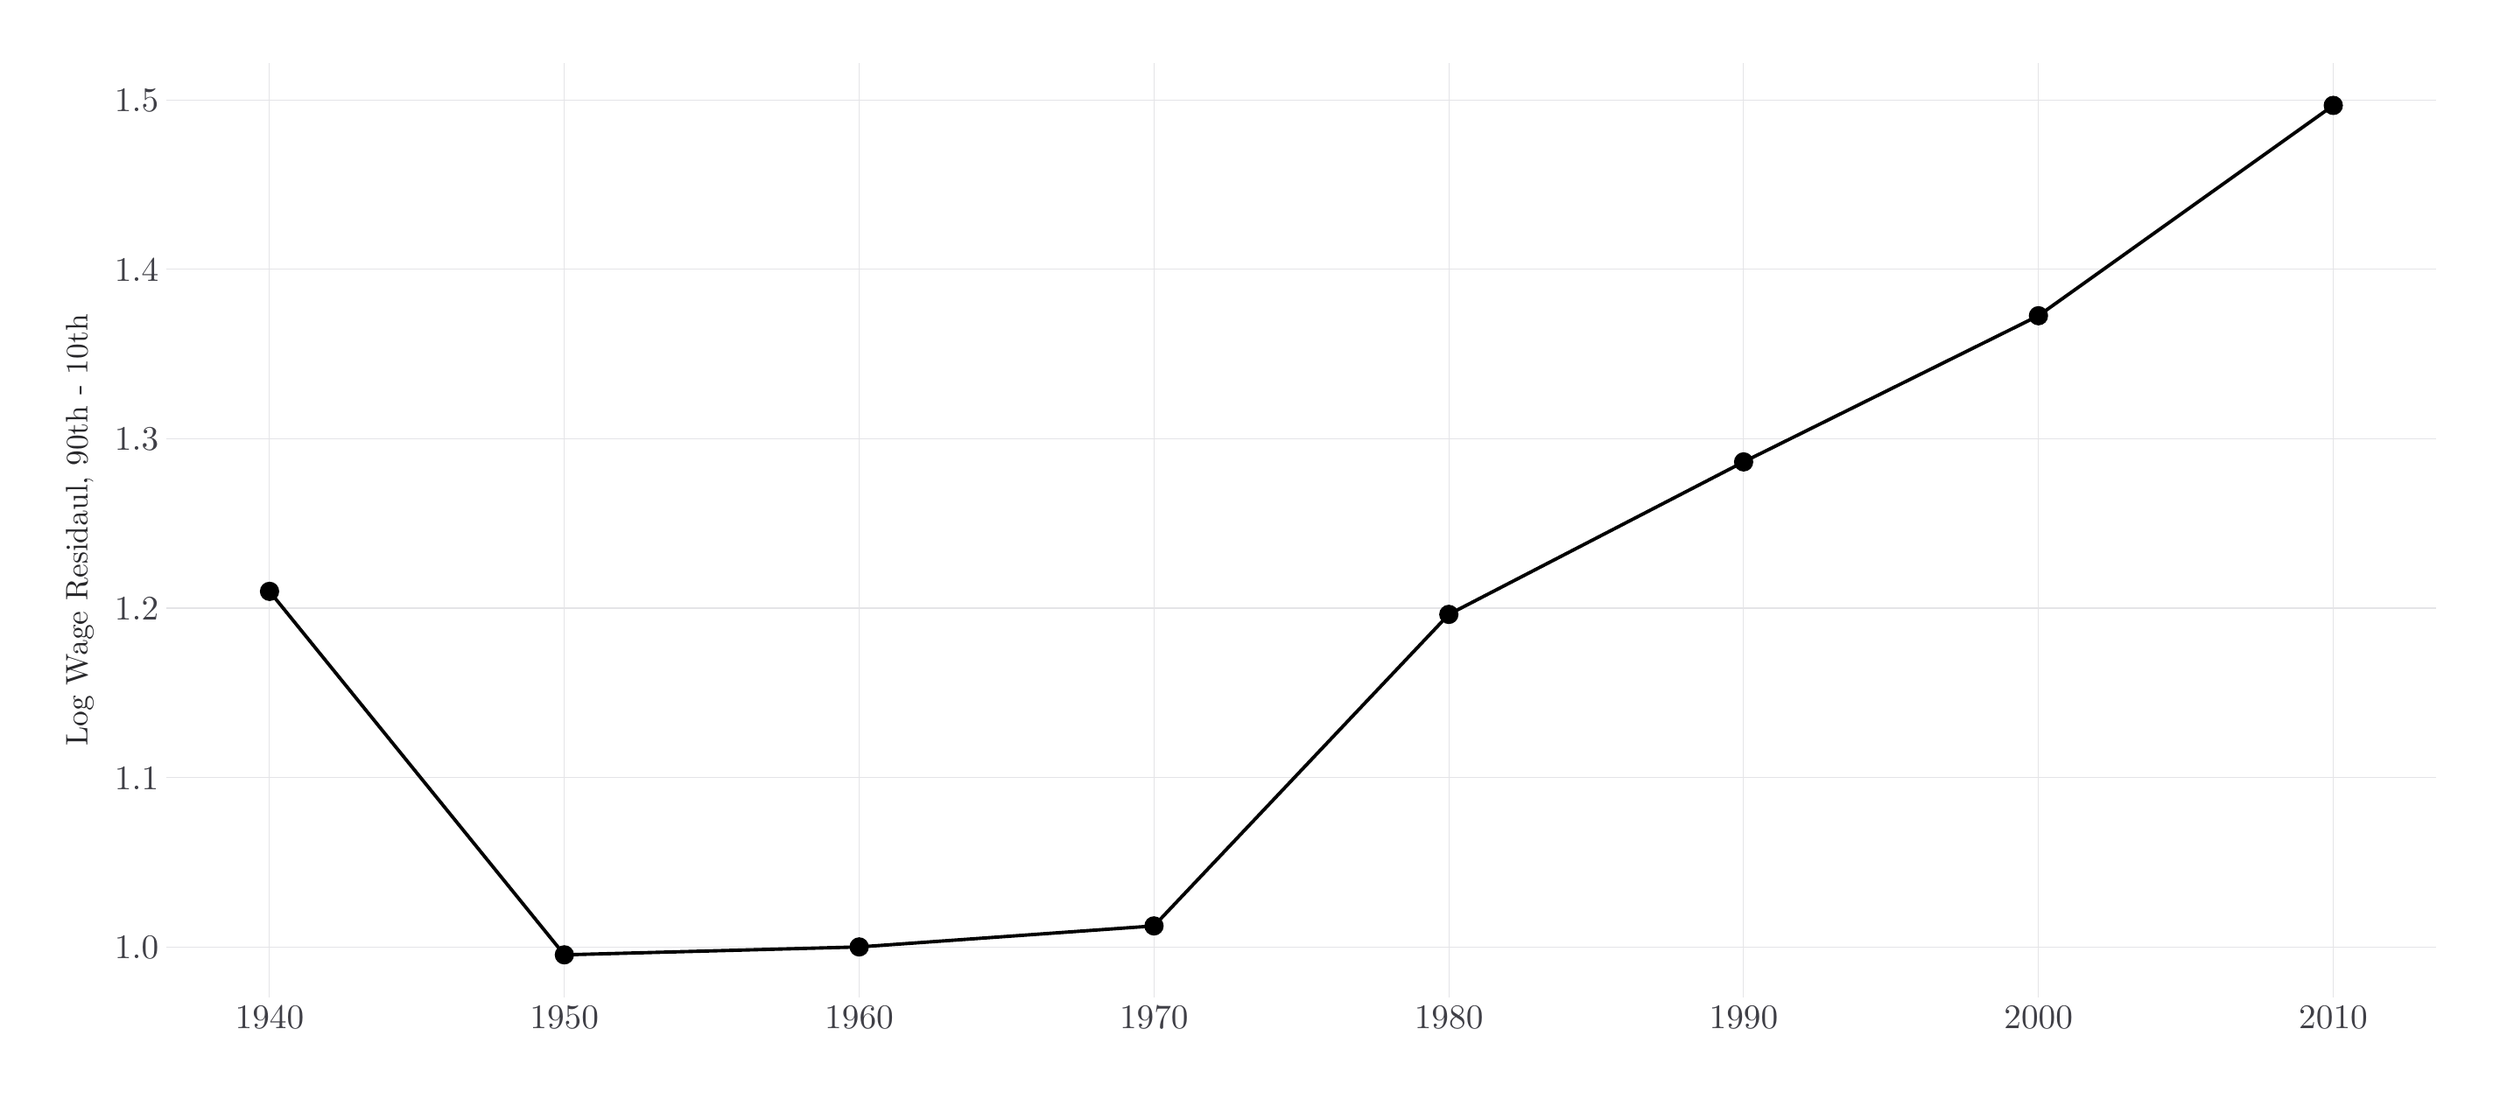
\begin{tikzpicture}[x=1pt,y=1pt]
\definecolor{fillColor}{RGB}{255,255,255}
\path[use as bounding box,fill=fillColor] (0,0) rectangle (1011.78,433.62);
\begin{scope}
\path[clip] (  0.00,  0.00) rectangle (1011.78,433.62);
\definecolor{drawColor}{RGB}{255,255,255}

\path[draw=drawColor,line width= 0.8pt,line join=round,line cap=round,fill=fillColor] (  0.00,  0.00) rectangle (1011.78,433.62);
\end{scope}
\begin{scope}
\path[clip] ( 58.67, 31.76) rectangle (995.78,417.62);
\definecolor{drawColor}{RGB}{255,255,255}
\definecolor{fillColor}{RGB}{255,255,255}

\path[draw=drawColor,line width= 0.8pt,line join=round,line cap=round,fill=fillColor] ( 58.67, 31.76) rectangle (995.78,417.62);
\definecolor{drawColor}{RGB}{228,228,231}

\path[draw=drawColor,line width= 0.4pt,line join=round] ( 58.67, 52.53) --
	(995.78, 52.53);

\path[draw=drawColor,line width= 0.4pt,line join=round] ( 58.67,122.51) --
	(995.78,122.51);

\path[draw=drawColor,line width= 0.4pt,line join=round] ( 58.67,192.48) --
	(995.78,192.48);

\path[draw=drawColor,line width= 0.4pt,line join=round] ( 58.67,262.45) --
	(995.78,262.45);

\path[draw=drawColor,line width= 0.4pt,line join=round] ( 58.67,332.42) --
	(995.78,332.42);

\path[draw=drawColor,line width= 0.4pt,line join=round] ( 58.67,402.40) --
	(995.78,402.40);

\path[draw=drawColor,line width= 0.4pt,line join=round] (101.27, 31.76) --
	(101.27,417.62);

\path[draw=drawColor,line width= 0.4pt,line join=round] (222.97, 31.76) --
	(222.97,417.62);

\path[draw=drawColor,line width= 0.4pt,line join=round] (344.67, 31.76) --
	(344.67,417.62);

\path[draw=drawColor,line width= 0.4pt,line join=round] (466.37, 31.76) --
	(466.37,417.62);

\path[draw=drawColor,line width= 0.4pt,line join=round] (588.08, 31.76) --
	(588.08,417.62);

\path[draw=drawColor,line width= 0.4pt,line join=round] (709.78, 31.76) --
	(709.78,417.62);

\path[draw=drawColor,line width= 0.4pt,line join=round] (831.48, 31.76) --
	(831.48,417.62);

\path[draw=drawColor,line width= 0.4pt,line join=round] (953.18, 31.76) --
	(953.18,417.62);
\definecolor{drawColor}{RGB}{0,0,0}
\definecolor{fillColor}{RGB}{0,0,0}

\path[draw=drawColor,line width= 0.5pt,line join=round,line cap=round,fill=fillColor] (101.27,199.40) circle (  3.73);

\path[draw=drawColor,line width= 0.5pt,line join=round,line cap=round,fill=fillColor] (222.97, 49.30) circle (  3.73);

\path[draw=drawColor,line width= 0.5pt,line join=round,line cap=round,fill=fillColor] (344.67, 52.56) circle (  3.73);

\path[draw=drawColor,line width= 0.5pt,line join=round,line cap=round,fill=fillColor] (466.37, 61.24) circle (  3.73);

\path[draw=drawColor,line width= 0.5pt,line join=round,line cap=round,fill=fillColor] (588.08,189.89) circle (  3.73);

\path[draw=drawColor,line width= 0.5pt,line join=round,line cap=round,fill=fillColor] (709.78,252.87) circle (  3.73);

\path[draw=drawColor,line width= 0.5pt,line join=round,line cap=round,fill=fillColor] (831.48,313.23) circle (  3.73);

\path[draw=drawColor,line width= 0.5pt,line join=round,line cap=round,fill=fillColor] (953.18,400.08) circle (  3.73);

\path[draw=drawColor,line width= 1.4pt,line join=round] (101.27,199.40) --
	(222.97, 49.30) --
	(344.67, 52.56) --
	(466.37, 61.24) --
	(588.08,189.89) --
	(709.78,252.87) --
	(831.48,313.23) --
	(953.18,400.08);
\end{scope}
\begin{scope}
\path[clip] (  0.00,  0.00) rectangle (1011.78,433.62);
\definecolor{drawColor}{RGB}{63,63,70}

\node[text=drawColor,anchor=base east,inner sep=0pt, outer sep=0pt, scale=  1.42] at ( 55.47, 47.64) {1.0};

\node[text=drawColor,anchor=base east,inner sep=0pt, outer sep=0pt, scale=  1.42] at ( 55.47,117.61) {1.1};

\node[text=drawColor,anchor=base east,inner sep=0pt, outer sep=0pt, scale=  1.42] at ( 55.47,187.58) {1.2};

\node[text=drawColor,anchor=base east,inner sep=0pt, outer sep=0pt, scale=  1.42] at ( 55.47,257.55) {1.3};

\node[text=drawColor,anchor=base east,inner sep=0pt, outer sep=0pt, scale=  1.42] at ( 55.47,327.53) {1.4};

\node[text=drawColor,anchor=base east,inner sep=0pt, outer sep=0pt, scale=  1.42] at ( 55.47,397.50) {1.5};
\end{scope}
\begin{scope}
\path[clip] (  0.00,  0.00) rectangle (1011.78,433.62);
\definecolor{drawColor}{RGB}{63,63,70}

\node[text=drawColor,anchor=base,inner sep=0pt, outer sep=0pt, scale=  1.42] at (101.27, 18.76) {1940};

\node[text=drawColor,anchor=base,inner sep=0pt, outer sep=0pt, scale=  1.42] at (222.97, 18.76) {1950};

\node[text=drawColor,anchor=base,inner sep=0pt, outer sep=0pt, scale=  1.42] at (344.67, 18.76) {1960};

\node[text=drawColor,anchor=base,inner sep=0pt, outer sep=0pt, scale=  1.42] at (466.37, 18.76) {1970};

\node[text=drawColor,anchor=base,inner sep=0pt, outer sep=0pt, scale=  1.42] at (588.08, 18.76) {1980};

\node[text=drawColor,anchor=base,inner sep=0pt, outer sep=0pt, scale=  1.42] at (709.78, 18.76) {1990};

\node[text=drawColor,anchor=base,inner sep=0pt, outer sep=0pt, scale=  1.42] at (831.48, 18.76) {2000};

\node[text=drawColor,anchor=base,inner sep=0pt, outer sep=0pt, scale=  1.42] at (953.18, 18.76) {2010};
\end{scope}
\begin{scope}
\path[clip] (  0.00,  0.00) rectangle (1011.78,433.62);
\definecolor{drawColor}{RGB}{39,39,42}

\node[text=drawColor,rotate= 90.00,anchor=base,inner sep=0pt, outer sep=0pt, scale=  1.28] at ( 26.06,224.69) {Log Wage Residaul, 90th - 10th};
\end{scope}
\end{tikzpicture}
